%%%%%%%%%%%%%%%%%%%%%%%%%%%%%%%%%%%%%%%%%%%%%%%%%%%%%%%%%%%%%%%%%%%%%%%%%%%%%%%%%%%%%%%%%%
%%%%%%%%%%%%
%%%%%%%%%%%% This report template was constructed by
%%%%%%%%%%%% Fredrik Hedström & Jörg Schminder, Linköping university, 2016
%%%%%%%%%%%% and correspond to LiU's official layout for Master-These reports. 
%%%%%%%%%%%%
%%%%%%%%%%%%%%%%%%%%%%%%%%%%%%%%%%%%%%%%%%%%%%%%%%%%%%%%%%%%%%%%%%%%%%%%%%%%%%%%%%%%%%%%%%

\documentclass[11pt,a4paper,twoside,oneside]{article}

    %\usepackage{fontspec}
    %\setmainfont{Calibri} 

\usepackage{nameref}
\usepackage[left=3.5cm, right=3.5cm, top=3.5cm, bottom=3.5cm]{geometry} 
\usepackage{multirow}
\usepackage{graphicx}
\graphicspath{{./images/}}
\usepackage[latin1]{inputenc}
%\usepackage{enumerate}
\usepackage{setspace}
\usepackage{boxedminipage}
\usepackage{longtable}
\usepackage{booktabs}
\usepackage{ctable}
\usepackage[font=footnotesize, font+=bf, skip=5pt]{caption}
%\usepackage{subfig}
\usepackage{float}
\usepackage[super]{nth}
\usepackage{blindtext}
\usepackage{mathtools}
\usepackage{hyperref}
\usepackage{epstopdf}
\usepackage{bibunits}
\usepackage{sectsty}
\usepackage{titlesec}

\titleformat*{\section}{\Huge\bfseries}
\titleformat*{\subsection}{\LARGE\bfseries}
\titleformat*{\subsubsection}{\Large\bfseries}
\titleformat*{\paragraph}{\large\bfseries}

\usepackage{combelow}
\usepackage{enumitem}
\usepackage{siunitx}
%\usepackage{paralist}
\usepackage{enumitem}
\usepackage{subcaption}
\usepackage{hyperref}

\newlength{\twosubht}
\newsavebox{\twosubbox}


\usepackage{adjustbox}
\usepackage{array}
\usepackage{multirow}
\newcolumntype{L}[1]{>{\raggedright\let\newline\\\arraybackslash\hspace{0pt}}m{#1}}
\newcolumntype{C}[1]{>{\centering\let\newline\\\arraybackslash\hspace{0pt}}m{#1}}
\newcolumntype{R}[1]{>{\raggedleft\let\newline\\\arraybackslash\hspace{0pt}}m{#1}}

\newcommand\T{\rule{0pt}{2.2ex}} % Top strut
\newcommand\B{\rule[-0.9ex]{0pt}{0pt}} % Bottom strut
\newcommand{\ra}[1]{\renewcommand{\arraystretch}{#1}}



%\defaultbibliography{references.bib}
%\defaultbibliographystyle{vancouver}

\begin{document}
%\begin{bibunit}[plain]
%%%%%%%%%%%%%%%%%%%%%%%%%%%%%%%%%%%%%%%%%%%%%%%%%%%%%%%%%%%%%%%%%%%%%%%%%%%%%%%%%%%%%%%%%%
%%%%%%%%%%%%
%%%%%%%%%%%%    											Title page 1
%%%%%%%%%%%%
%%%%%%%%%%%%%%%%%%%%%%%%%%%%%%%%%%%%%%%%%%%%%%%%%%%%%%%%%%%%%%%%%%%%%%%%%%%%%%%%%%%%%%%%%%

\begin{titlepage}
\newgeometry{left=1.5cm, right=1.5cm, top=0cm, bottom=.9cm} 
	\vspace*{2.5cm}
	\noindent \hspace{3.3cm} 
	{\Huge\textbf{A model aircraft    \\
	\hspace*{3.1cm} CFD investigation} \par}
	
	\vspace{1cm}
	\noindent \hspace{3.5cm} 
	{\Large\textbf{TMMV17 Aircraft Aerodynamics - Project Course}}
	
	\vspace{1.6cm}
	\noindent \hspace{3.7cm}{\large \textbf{Adrian Aru\cb{s}tei (adrar156)}}
	
		
\vspace{7cm}
\begin{figure}[h]
 \centering
	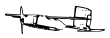
\includegraphics[trim = {-3cm 0 0 0} , clip, width=0.6\textwidth]{lineart.eps}
 \end{figure}
 
    \vfill
    \noindent
		
    \begin{minipage}{6.2cm}
    \includegraphics*[width=6.9cm]{LiuLogo.eps}
    \end{minipage}\hfill
    \begin{minipage}{10cm}
    \begin{onehalfspacing}
        \raggedleft
        Link\"oping University\\
        Division of Applied Thermodynamics and Fluid Mechanics\\
        Final Report $|$ 2019-01-18 \\%
        \end{onehalfspacing}
    \end{minipage}
 \restoregeometry

\end{titlepage}
\restoregeometry


%%%%%%%%%%%%%%%%%%%%%%%%%%%%%%%%%%%%%%%%%%%%%%%%%%%%%%%%%%%%%%%%%%%%%%%%%%%%%%%%%%%%%%%%%%
%%%%%%%%%%%%
%%%%%%%%%%%%    											Theses
%%%%%%%%%%%%
%%%%%%%%%%%%%%%%%%%%%%%%%%%%%%%%%%%%%%%%%%%%%%%%%%%%%%%%%%%%%%%%%%%%%%%%%%%%%%%%%%%%%%%%%%



%%%%%%%%%%%%%%%%%%%%%%%%%%%%%%%%  Chapter 1  %%%%%%%%%%%%%%%%%%%%%%%%%%%%%%%%%%%%%%%%%%%
\thispagestyle{plain}
\pagenumbering{arabic}

\section{Introduction}

\vspace{.6cm}

\noindent
This small project continues the work on the previously designed model aircraft from the TMAL07 course. The task was to build a prototype of a humanitarian aid UAV which is supposed to deliver a box with supplies at a target point and then return. The aircraft had to be cheap, simple and easy to manufacture. At the end of the course we had the chance to flight test the model. Because at the first flight the aircraft entered a flat spin and crashed, the present project tries elucidate the causes for this behaviour using CFD simulations on the model. By varying the angle of attack or sideslip angle it is expected that the aerodynamic moments will reflect the stability. 

Another purpose is related to the use of CFD in conceptual design. Since the payload is carried inside the fuselage, the question is whether cargo doors should be built or not. In other words, the project aims are as follows:
\begin{itemize} \setlength\itemsep{0em}
  \item[$-$] create a CFD model to study the performance of the UAV if a door is present at the bottom of the fuselage;
  \item[$-$] investigate the static stability of the aircraft, especially the lateral-directional stability; 
  \item[$-$] determine the influence of the vertical tail on the directional stability. How much should the vertical tail be enlarged to make the airplane stable?
\end{itemize}

One of the biggest limitations is that there is no validation data available from the previous course. The accent was put on manufacturing the prototype, so there were no flight parameters recorded or monitored. Furthermore, due to time constraints, only the longitudinal stability was checked and the sizing of the vertical tail was made by rules of thumb (like most of the aircraft). This represents a major weakness and as a consequence most of the teams had stability problems with their models.   





%%%%%%%%%%%%%%%%%%%%%%%%%%%%%%%%  Chapter 3  %%%%%%%%%%%%%%%%%%%%%%%%%%%%%%%%%%%%%%%%%%%
\clearpage
\thispagestyle{plain}

\section{Method}
\vspace{.6cm}

\subsection{Geometry preparation}

First, the geometry from the CAD had to be adapted for CFD simulations. This meant that all small details and edges were removed leaving only the main features (see Figures \ref{fig:geomd} and \ref{fig:geomc}). Of course this step introduces another set of uncertainties in our study. 

\begin{figure}[bp]
\sbox\twosubbox{%
  \resizebox{\dimexpr1\textwidth-1em}{!}{%
    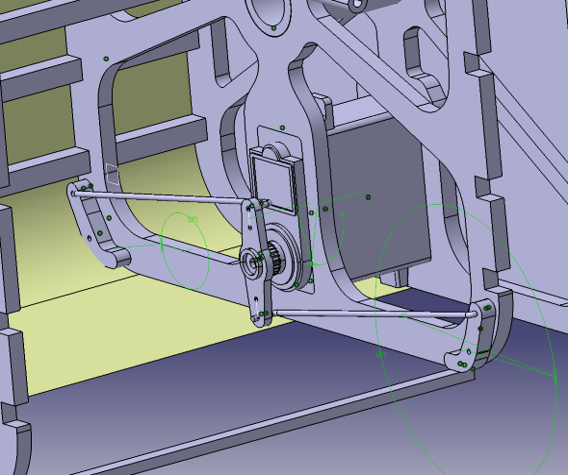
\includegraphics[height=3cm]{geomd.png}%
    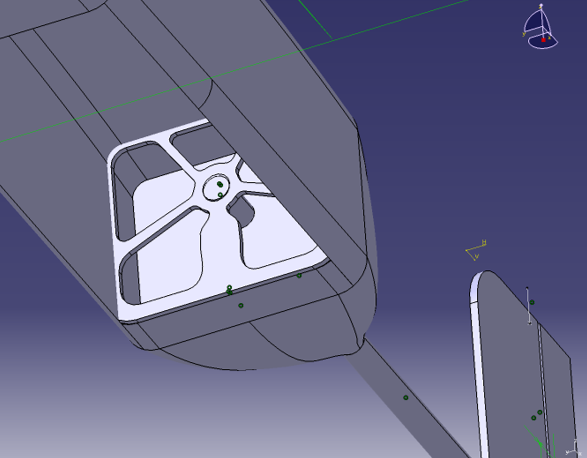
\includegraphics[height=3cm]{geomc.png}%
  }%
}
\setlength{\twosubht}{\ht\twosubbox}

\centering

\captionbox{CAD geometry. \label{fig:geomd}}{%
  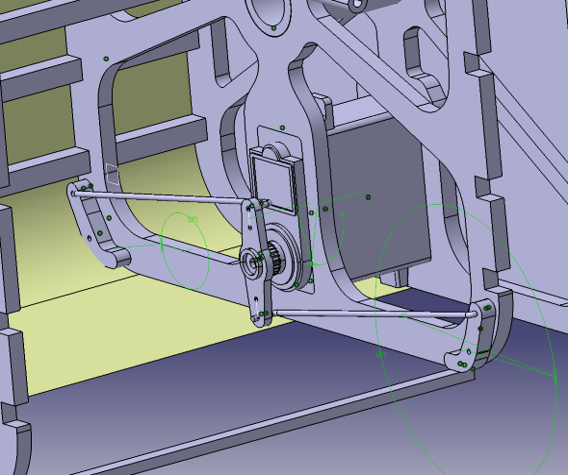
\includegraphics[height=0.9\twosubht]{geomd.png}%
}  \hfill
\captionbox{All the unnecessary details were removed. \label{fig:geomc}}{%
  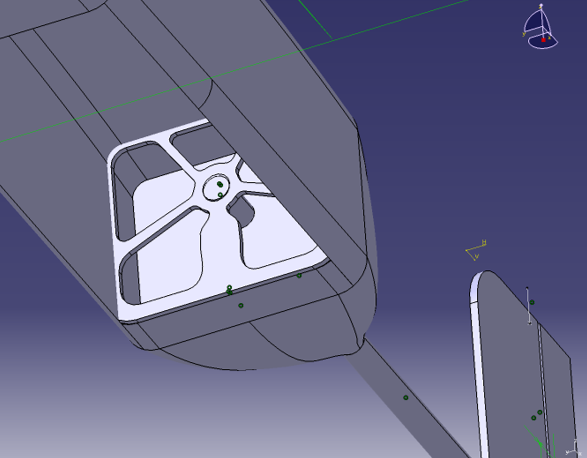
\includegraphics[height=0.9\twosubht]{geomc.png}%
}  
\end{figure}

Once the CAD geometry was ready, the Boolean operations to obtain the flow domain were done in ANSYS DesignModeler after rotations were applied around the predicted center of gravity from CAD. In this way the angle of attack and sideslip angle could be easily varied as parameters in Workbench. Furthermore, the control surfaces rotations were also parametrized because the stability study was to be performed around an equilibrium point, so the aircraft had to be trimmed. The rectangular domain can be seen in Figure \ref{dms}. For the first project aim, the geometries prepared can be seen in Figure \ref{desc}.

\begin{figure}%[htbp]
 \centering
	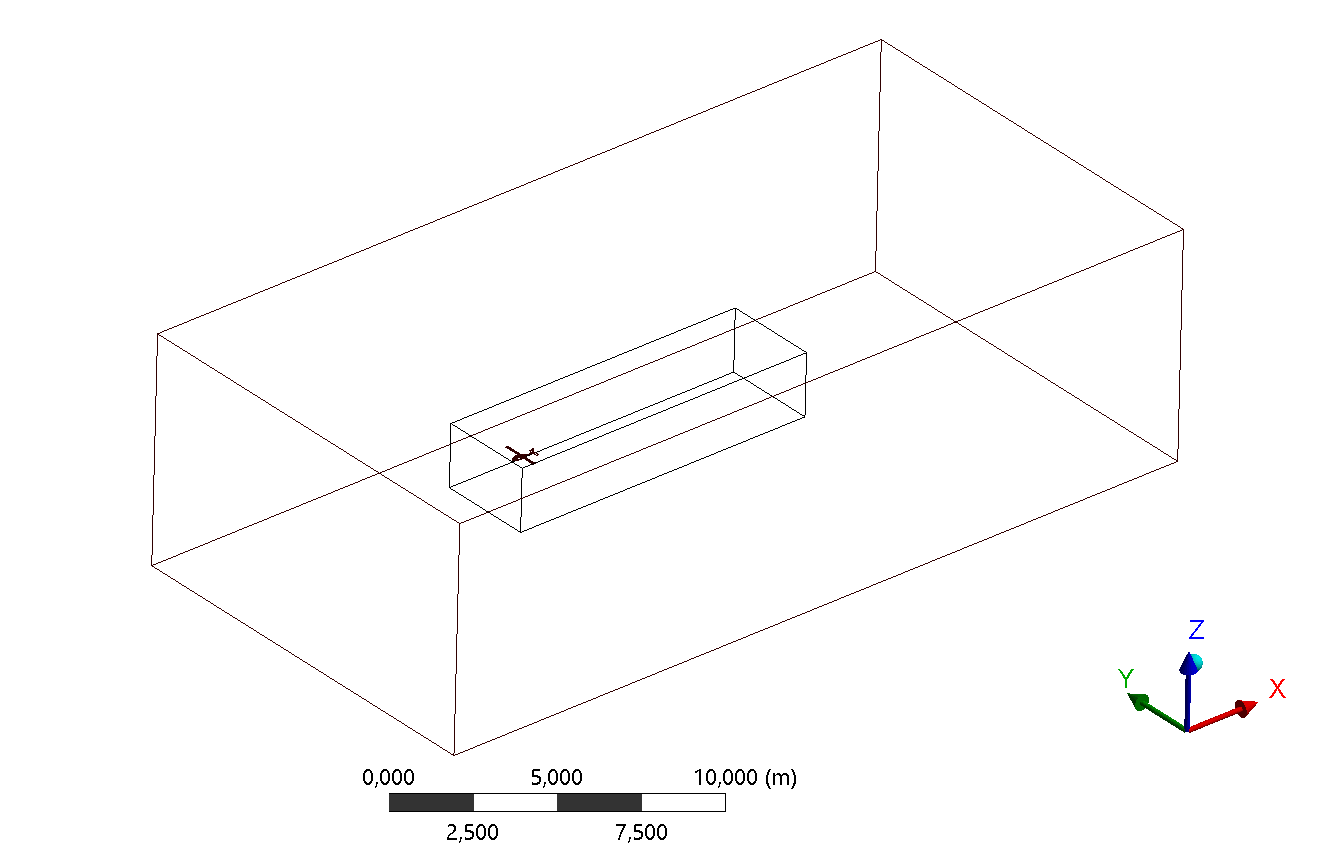
\includegraphics[width=0.9\textwidth]{DomainSize.PNG}
	\captionsetup{width=.9\linewidth}
	\caption{Flow domain with a body of influence around and downstream the model. The sizes are, in body lengths, 8 in height, 14 in width, 8 upstream and 20 downstream of aircraft. \label{dms}}
 \end{figure}

\begin{figure}%[htbp]
 \centering
	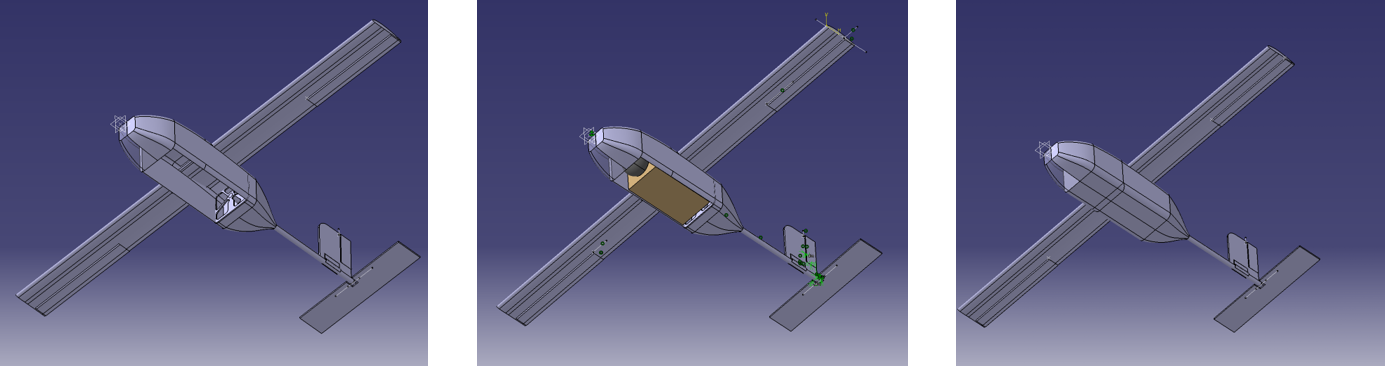
\includegraphics[width=1\textwidth]{descas.png}
	\caption{Design cases to study: without box, with box, with doors (perfectly closed). \label{desc}} 
 \end{figure}
 
\subsection{Mesh generation and solver set-up}

Regarding the solver set-up, the turbulence model used was Spalart-Allmaras. The choice was made because, being a one-equation model, it performs slightly faster than k-omega for example. Robustness and time efficiency had to be kept in mind since the cell count was high and the available computational power limited. The SA model is a low-Reynolds number model and is expected to give the best results when the boundary layer is solved all the way to the wall, i.e. when $y+\approx1$. However, in our case a $y+$ value of 1 was not possible to achieve due to computational limitations. Another way to reduce the wall $y+$ is to decrease the flow velocity. The velocity chosen for this study is $\SI{14}{\m\per\s}$ which is close to the expected stall velocity of $\SI{12}{\m\per\s}$ calculated in the previous course. A plausible flying condition was wanted to be simulated so the velocity was not reduced further. In FLUENT the SA model was made insensitive to $y+$ values through the use of Enhanced wall functions, so it will work on coarser meshes too. This is the default behaviour for SA model (as mentioned in ch. 4.16.1 in the FLUENT documentation \cite{ansys}).

The boundary conditions used were symmetry on the sides of the domain, inlet velocity and pressure outlet and no-slip wall on the model. These conditions mimic the flight in a free airstream with a fixed velocity, far away from any obstacles. The domain has to be large enough such that the boundaries effect is negligible. For example the flow might be artificially accelerated due to the blockage effect if the domain cross-sectional area is too small.

The numerical schemes used were second order for the pressure equation for improved accuracy. No checkerboard patterns were observed in the solutions. The momentum and turbulence equations were discretized with a first-order scheme to avoid oscillations in the interest variables (lift, drag and moments). The pressure-velocity scheme used was set to coupled.

The convergence criteria was set to 1e-5 for the un-normalized scaled residuals. By the time the residuals dropped to this value it was observed that the integrated quantities like lift and drag are well converged. This usually happened in around 70 iterations so a limit of 150 iterations was set, although never reached. All simulations had a similar behaviour regarding the residuals. With the first order schemes used no convergence problems were encountered. Higher order schemes sometimes did not completely converge due to the flow instability at such high angles of attack (almost near stall), so they were not used.



\subsubsection{Mesh sensitivity}
 The mesh sensitivity in Table \ref{table:meshs} was conducted for a \ang{5} degree angle of attack at a velocity of $\SI{14}{\m\per\s}$. It can be seen that the pitch moment is almost 0 (one equilibrium condition) and that the lift and drag variations are relatively small. Considering the extra time required for the finer mesh, it was decided to use the settings for the coarse mesh in further simulations.

\begin{table}[hbp]
\caption{Mesh sensitivity study.}
\centering
\begin{adjustbox}{center}
\ra{1.3}
\begin{tabular}{l l l l l}
\toprule %inserts double horizontal lines
Cell no. & Drag [\si{N}] & Lift [\si{N}] & Pitch mom. [\si{\N\m}] & Time [\si{h}] \\ \midrule
\num{5693581} & 1.404 (+1.49\%)  &	12.034 (-4.04\%) &  +0.00779 &	4.2     \\
  \num{9021750} & 1.384 \phantom{(+1.49\%)}  & 12.542 \phantom{(-4.04\%)}	&  -0.000763	& 8.3	\\ \bottomrule
\end{tabular}
\end{adjustbox}
\label{table:meshs}
\end{table}


\subsection{With propeller or not?}
Initially it was planned that all the simulations should be done in the absence of the propeller for simplicity reasons. After the first simulations it was concluded that the propeller must have had a significant role in stability, so it had to be included. Then, it was realized that when the airplane crashed after launch it actually had the payload inside. Thus, the initial simulation cases ware actually a little bit far from reality. So, the payload and propeller were included in the last part of this project. 

There are 4 main ways to simulate a rotating propeller in Fluent:
\begin{itemize}
  \item[$-$] 3D Fan Zones have the advantage that the propeller geometry is not needed. However, a pressure jump or a fan curve must be provided;
  \item[$-$] Moving Reference Frames (also known as the "frozen rotor approach") is a steady state approximation which solves the moving reference frame equations in the cell zones with a specified rotational velocity. Note that here the mesh does not move; 
  \item[$-$] Mixing Plane Model is similar to Moving Reference Frames but it overcomes some of its limitations, for example in turbo-machinery applications. The main difference is how the variables are treated at the interface;
  \item[$-$] Sliding Mesh Model is necessarily unsteady due to the motion of the mesh with time.
\end{itemize}

The approach chosen is the Moving Reference Frame (MRF) being easy to implement. A 2 blade 12x4 propeller model (similar to the real one) was taken from the free CAD library \href{www.grabcad.com}{GrabCAD} and subtracted from of a cylinder domain, the cell zone in which the moving reference frame equations will be solved (check Figure \ref{mesh}). This cylinder follows the body rotations together with the aircraft. Being set as a single "part" in DesignModeler with the whole domain, the mesh is conformal, i.e. nodes at the interface between the 2 cell zones coincide. The rotational velocity was set to $\SI{672}{rad\per\s}$ (around $\SI{6417}{rpm}$), value which gives enough thrust to overcome the drag. The motor used in reality had a rotational velocity range between 6000 and $\SI{9000}{rpm}$ depending on the propeller and voltage supplied, so our determined value seems plausible. 

\begin{figure}%[htbp]
 \centering
	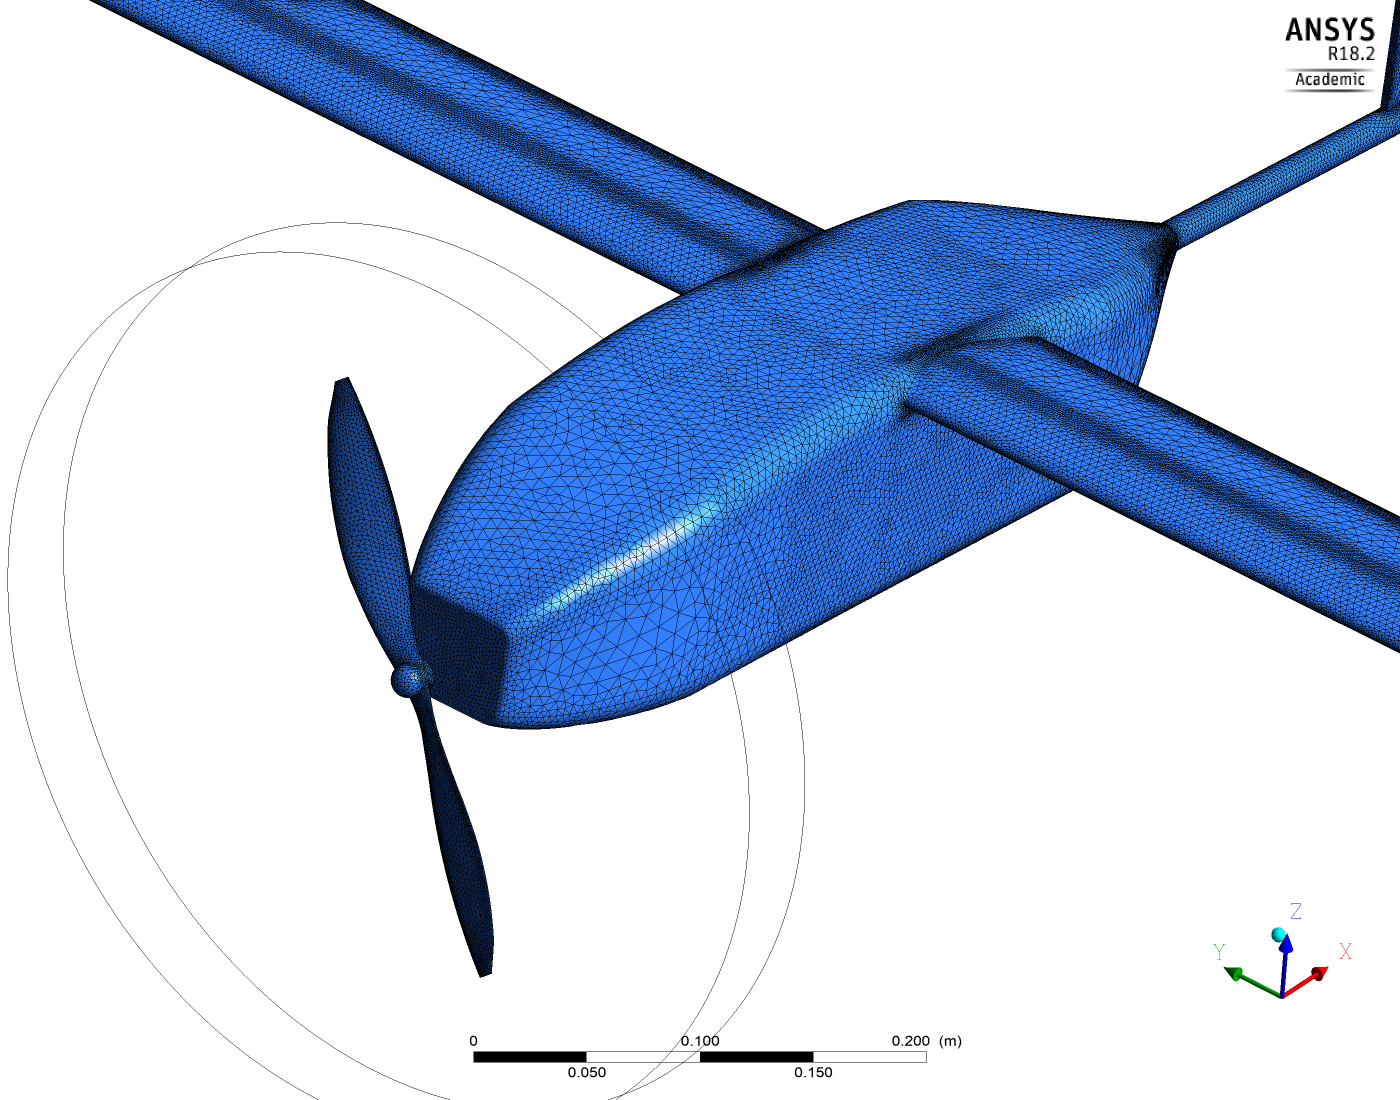
\includegraphics[width=0.9\textwidth]{Mesh.png}
	\caption{The propeller is inside a moving reference region. \label{mesh}} 
 \end{figure}
 
 
\subsection{A theoretically stable aircraft}
A statically stable aircraft will tend to return to its equilibrium position when disturbed. As summarized in \cite{stabi}, there are three main conditions for a statically stable aircraft:
\begin{itemize} \setlength\itemsep{0em}
  \item[$-$] Longitudinal: the slope of the pitch moment versus angle of attack to be negative, i.e. $C_{m_\alpha}<0$;
  \item[$-$] Directional: the slope of the yaw moment versus sideslip angle to be positive, i.e $C_{n_\beta}>0$; 
  \item[$-$] Lateral: the slope of the rolling moment versus sideslip angle to be negative, i.e. $C_{l_\beta}<0$; 
\end{itemize}
In our method, these conditions will be qualitatively verified for our UAV by using design points and varying the angle of attack and sideslip by a finite amount (usually one or two degrees).

Regarding the longitudinal neutral point, it is defined as the point about which the pitch moment does not change with a change in angle of attack. So the line which is flat (its derivative is 0) will correspond to the neutral point. This value will be compared with previous estimates. 
 
 
%%%%%%%%%%%%%%%%%%%%%%%%%%%%%%%%  Chapter 4  %%%%%%%%%%%%%%%%%%%%%%%%%%%%%%%%%%%%%%%%%%%
\clearpage
\thispagestyle{plain}

\section{Results}

\subsection{Performance in different configurations}
In Figure \ref{vdesc} a contour plot of velocities in the 3 design cases can be seen. When adding the box, the gap in the fuselage is filled and the main vortex blocked so the drag is reduced. There is still a flow around the box so drag could be reduced even more by sealing the fuselage with the help of a cargo door. From the Figure \ref{impld} we see that the best Lift/Drag improvement is around $\SI{21}{\m\per\s}$ which corresponds to a \ang{0} angle of attack (the wing is offsetted from the fuselage and cambered so it is still producing lift). 

\begin{figure}[h]
 \centering
	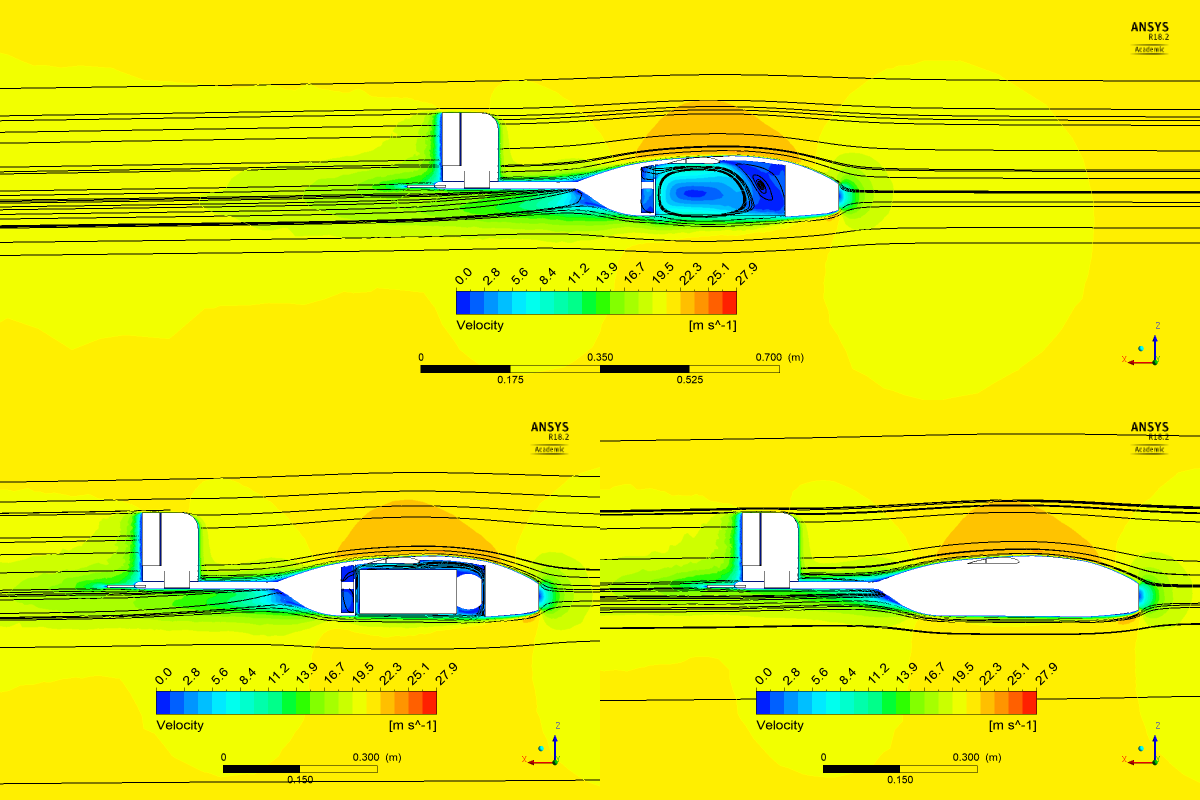
\includegraphics[width=1\textwidth]{VelStreamline3.png}
	\caption{Veloctity contour plot and streamlines for the three design cases. The box and doors block the recirculation inside the fuselage thus decreasing the drag. \label{vdesc}} 
 \end{figure}
 
 \begin{figure}%[t]
 \centering
	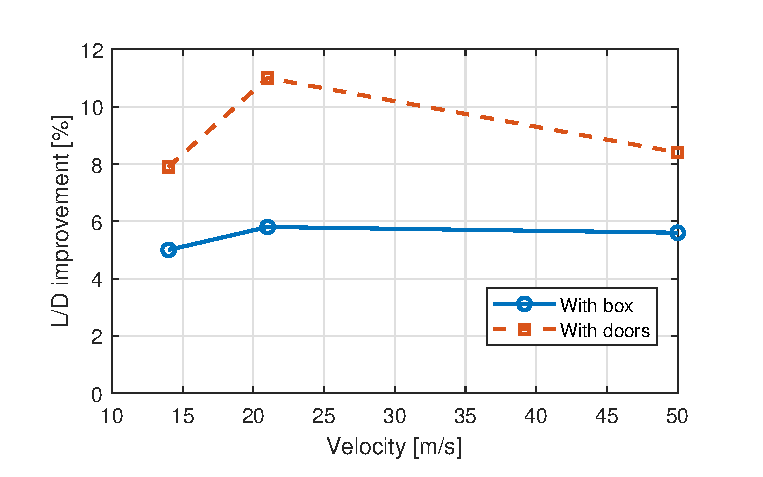
\includegraphics[width=0.7\textwidth]{desg.eps}	\captionsetup{width=0.7\linewidth}
	\caption{Lift/Drag improvement compared to the airplane without box. At $\SI{21}{\m\per\s}$ the L/D gain is the largest from the 3 cases tested. \label{impld}} 
 \end{figure}
 

\subsection{Longitudinal stability and neutral point}

To determine the longitudinal neutral point we take a look at the slopes of the curves in Figure \ref{np}. It is found to be $\SI{5}{cm}$ aft the center of gravity. With this value one can compute the position of neutral point as percentage of the mean aerodynamic chord and compare it with previous results. In Table \ref{table:np} we see that the classical formula is conservative (using it will result in a very stable design) and that the CFD result is very close to an estimation found in \cite{lab8}. Note that this neutral point position was obtained in the case without the propeller.

\begin{figure}%[htbp]
 \centering
	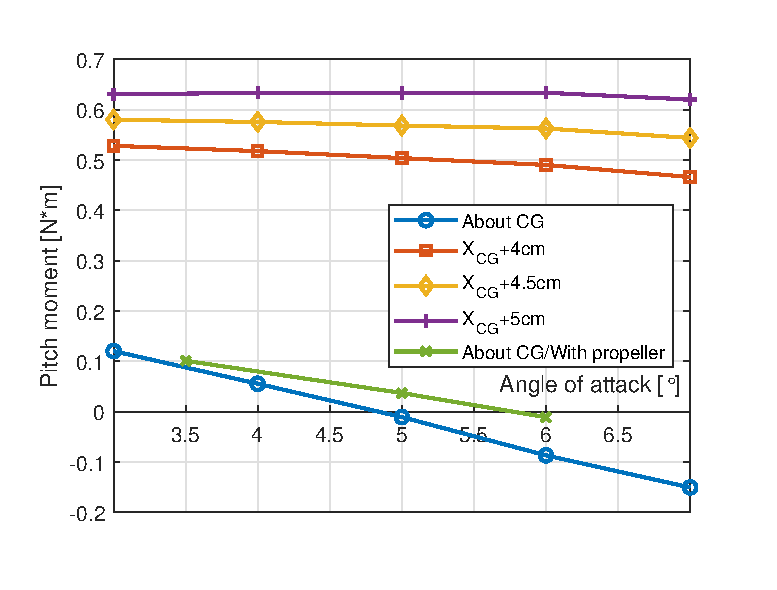
\includegraphics[width=0.7\textwidth]{pitmom.eps}
	\captionsetup{width=.7\linewidth}
	\caption{Graphical method to estimate the neutral point position and to check for static longitudinal stability. \label{np}} 
 \end{figure}


\begin{table}%[htbp]
\caption{Neutral point estimation comparison}
\centering
\begin{adjustbox}{center}
\ra{1.3}
\begin{tabular}{c l}
\toprule %inserts double horizontal lines
$x_{NP}$ as percentage of MAC & Formula \\ \midrule
67\% & in Eq. 11-26 in \cite{generalaviation}     \\
82\% & CFD, present result	\\
83\% & eq. 5 in \cite{lab8}\\
92\% & self deduced in TMAL06 \\\bottomrule
\end{tabular}
\end{adjustbox}
\label{table:np}
\end{table}


\subsection{Lateral-directional stability}

For the lateral-directional stability the yaw and roll moment are studied in relation with sideslip angle. In Figures \ref{yawmom} and \ref{rollmom} we see that the conditions for stability are generally respected for the airplane without propeller. However, a strange behaviour occurred in the rolling moment (large variations near the \ang{0}). This was tried to be tracked down to the flow features inside the fuselage who were starting to shift and rotate in new directions with a change in sideslip (as shown in Figures \ref{bet2yx} and \ref{bet2side}). Curiously, when adding the box and propeller these roll moment oscillations disappear and the aircraft becomes even more laterally stable. 
Not the same thing happens with the directional stability. The propeller has a destabilizing effect and the yaw moment slope even becomes slightly negative when it should be positive (see the green curve in Figure \ref{yawmom}). This happens due to the fact that the vertical tail is situated in the propeller slipstream which reduces its effectiveness of creating restoring yaw moment (this can be observed in Figures \ref{noprop} and \ref{withprop} by noticing the increase of velocity downstream the propeller).

\begin{figure}%[htbp]
\raggedleft
\makebox[1\textwidth][c]{%
\begin{minipage}{0.78\textwidth}
 \centering
	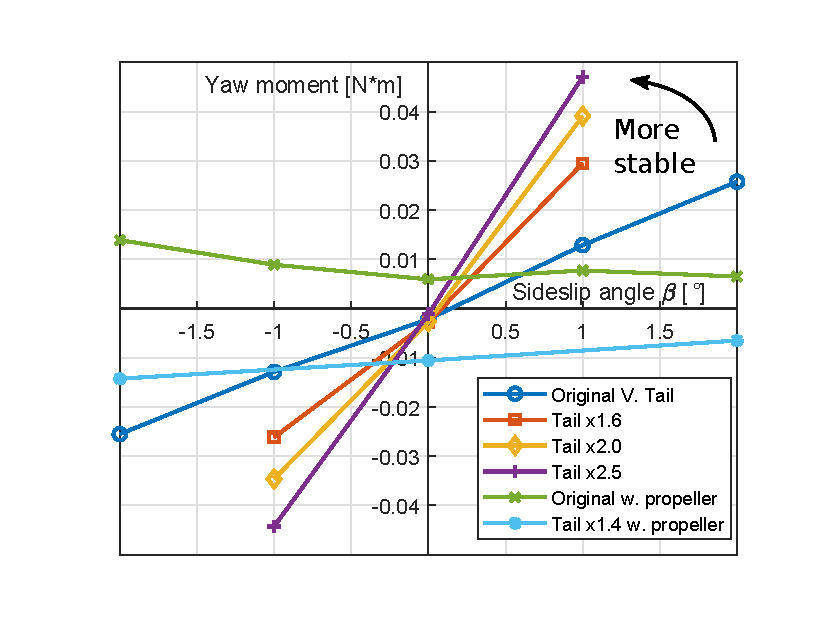
\includegraphics[trim = {0.4cm 0.4cm 0.1cm 0 }, clip, width=1\textwidth]{yawmom4.eps}
	\captionsetup{width=0.83\linewidth}
	\caption{Yawing moment with respect to sideslip angle. By inspecting the slopes of the curves, we see that the propeller is heavily destabilizing. \label{yawmom}} 
\end{minipage}%
\hspace{-1.1cm}
\begin{minipage}{0.78\textwidth}
	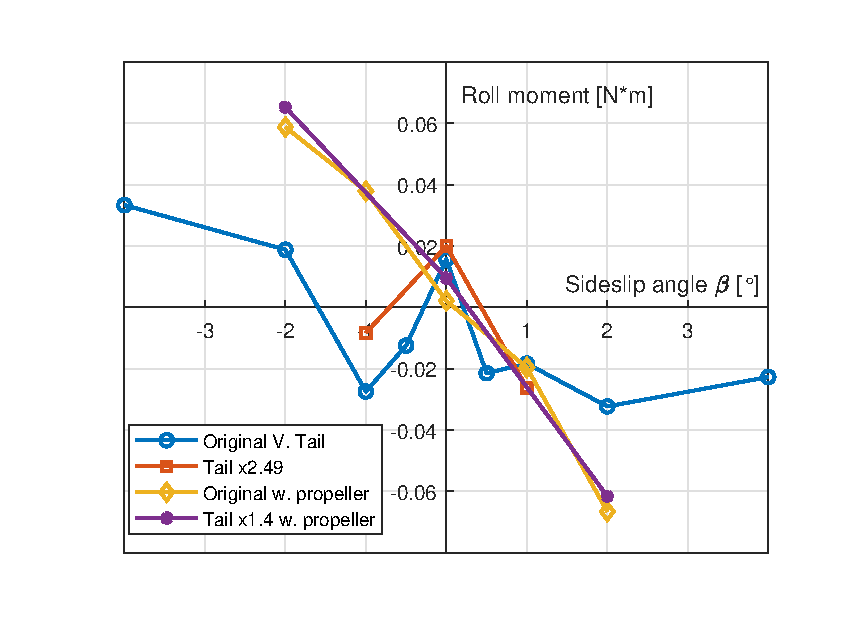
\includegraphics[trim = {0.5cm 0.4cm 0.3cm 0 }, clip, width=1\textwidth]{rollmom.eps}
	\captionsetup{width=0.83\linewidth}
	\caption{Rolling moment with respect to sideslip angle. Strange behaviour occurs around the \ang{0} angle when no propeller is present.  \label{rollmom}} 
 \end{minipage}}
\end{figure}

 
\begin{figure}%[htbp]
\raggedleft
\makebox[1\textwidth][c]{%
\begin{minipage}{0.6\textwidth}
  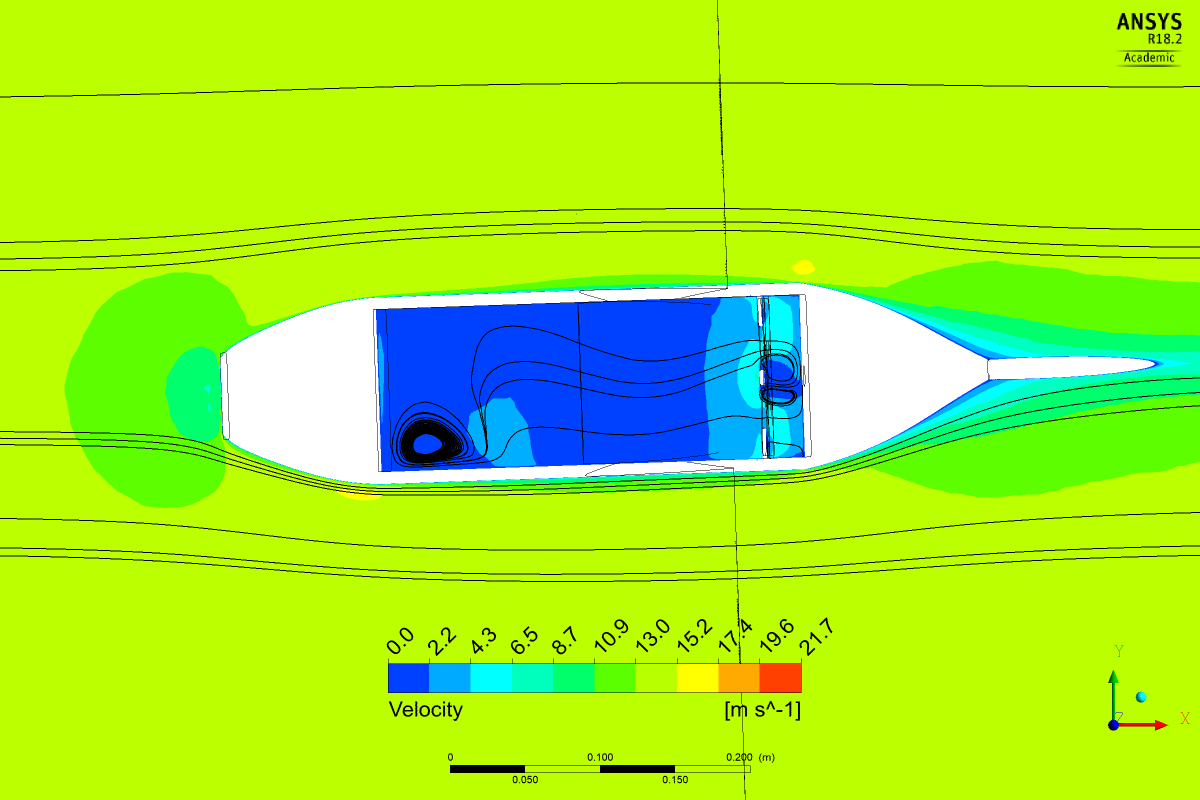
\includegraphics[trim = {6cm 0 8cm 3cm} , clip, width=1\linewidth]{Beta25AoaYX.png}
  \captionof{figure}{At a sideslip angle, the smaller vortex which can also be seen in Figure \ref{vdesc} moves sideways and starts spinning in the horizontal plane. \label{bet2yx}}
\end{minipage}%
\hspace{1cm}
\begin{minipage}{0.6\textwidth}
  %\centering
  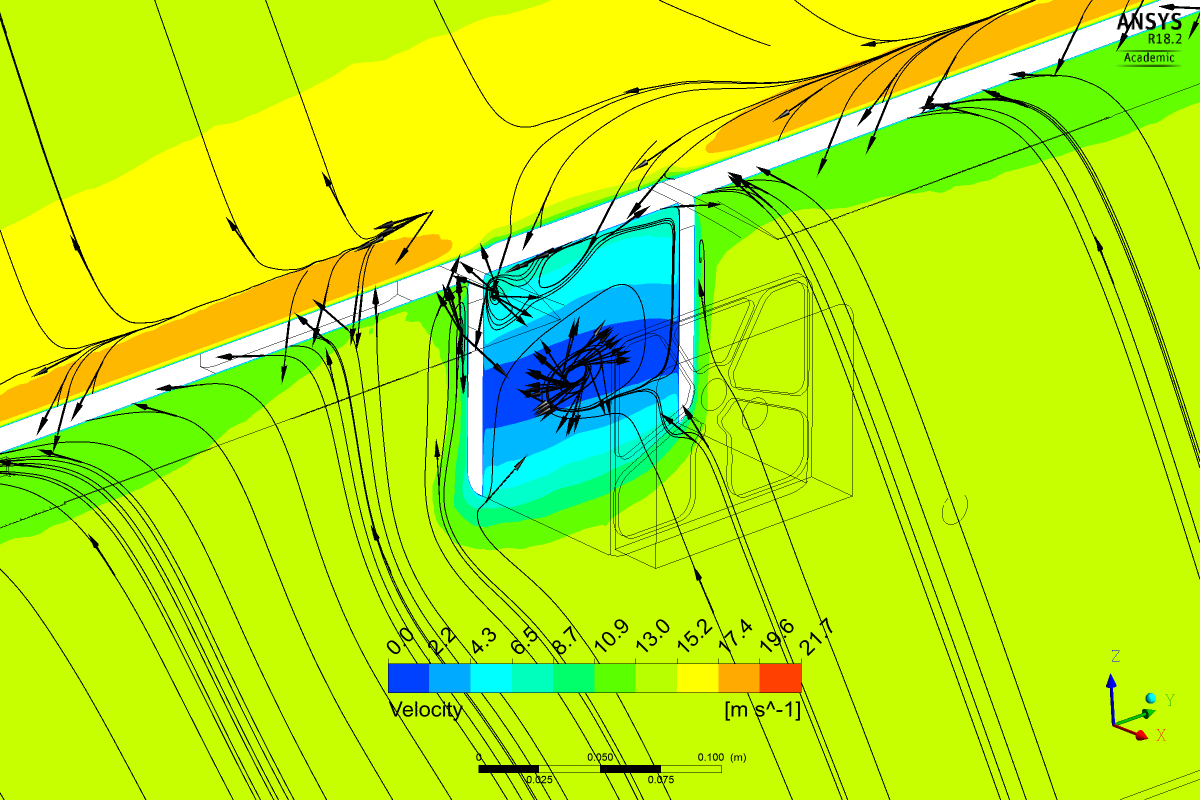
\includegraphics[trim = {6cm 0 8cm 3cm} , clip, width=1\linewidth]{Beta25Aoaplan03.png}
  \captionof{figure}{The sideslip angle gives a rolling motion to the main vortex in the fuselage. No conclusion was found to explain the oscillations in Fig.~\ref{rollmom}. \label{bet2side}}
 \end{minipage}}
\end{figure}

\begin{figure}%[htbp]
\raggedleft
\makebox[1\textwidth][c]{%
\begin{minipage}{0.6\textwidth}
  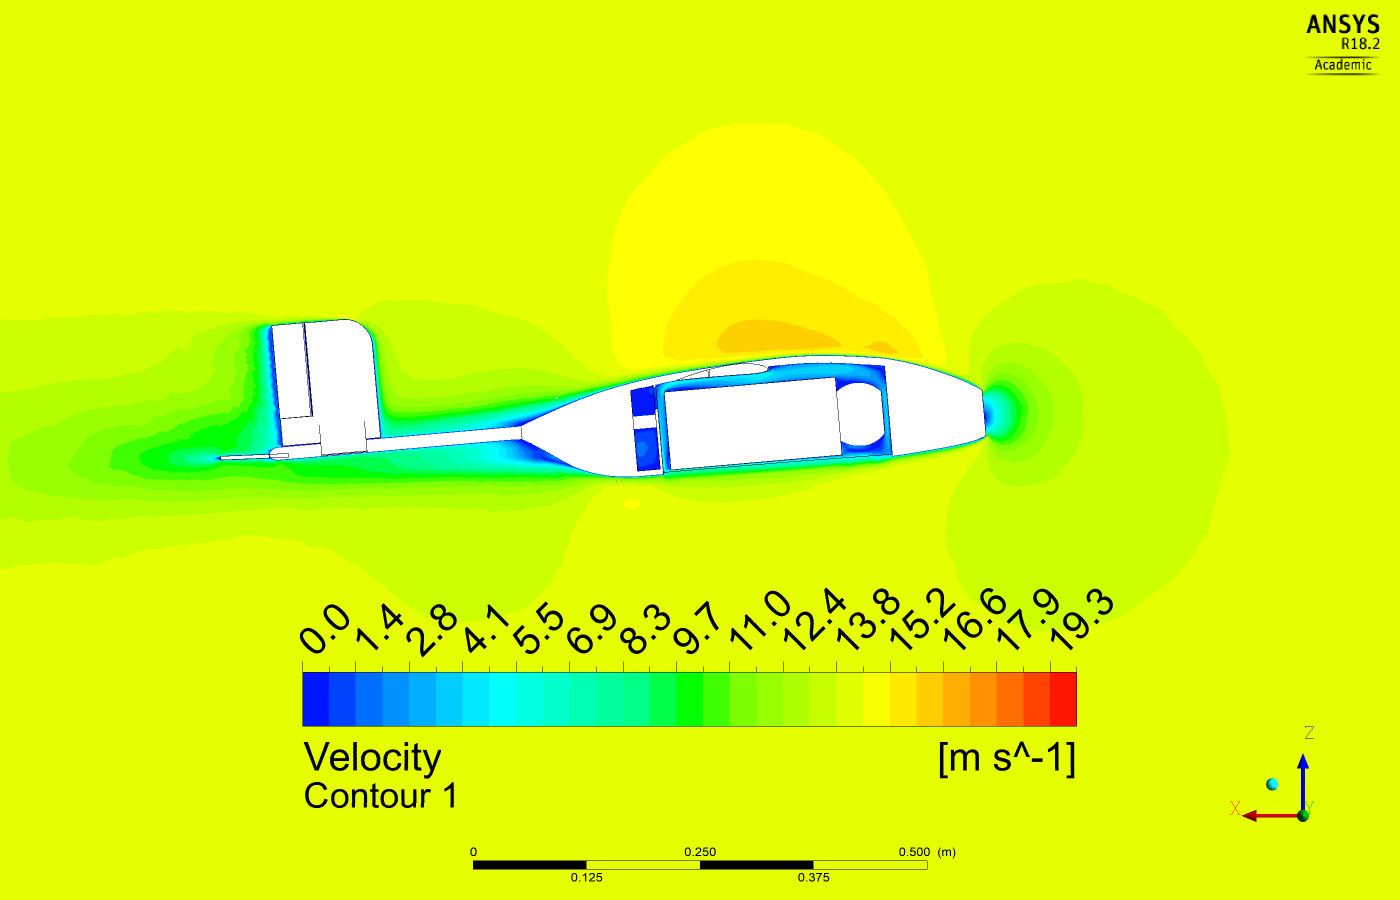
\includegraphics[trim = {6cm 0 8cm 3cm} , clip, width=1\linewidth]{velwbnoprop.png}
  \captionof{figure}{Midplane velocity contour, initial case. \label{noprop}}
\end{minipage}%
\hspace{1cm}
\begin{minipage}{0.6\textwidth}
  %\centering
  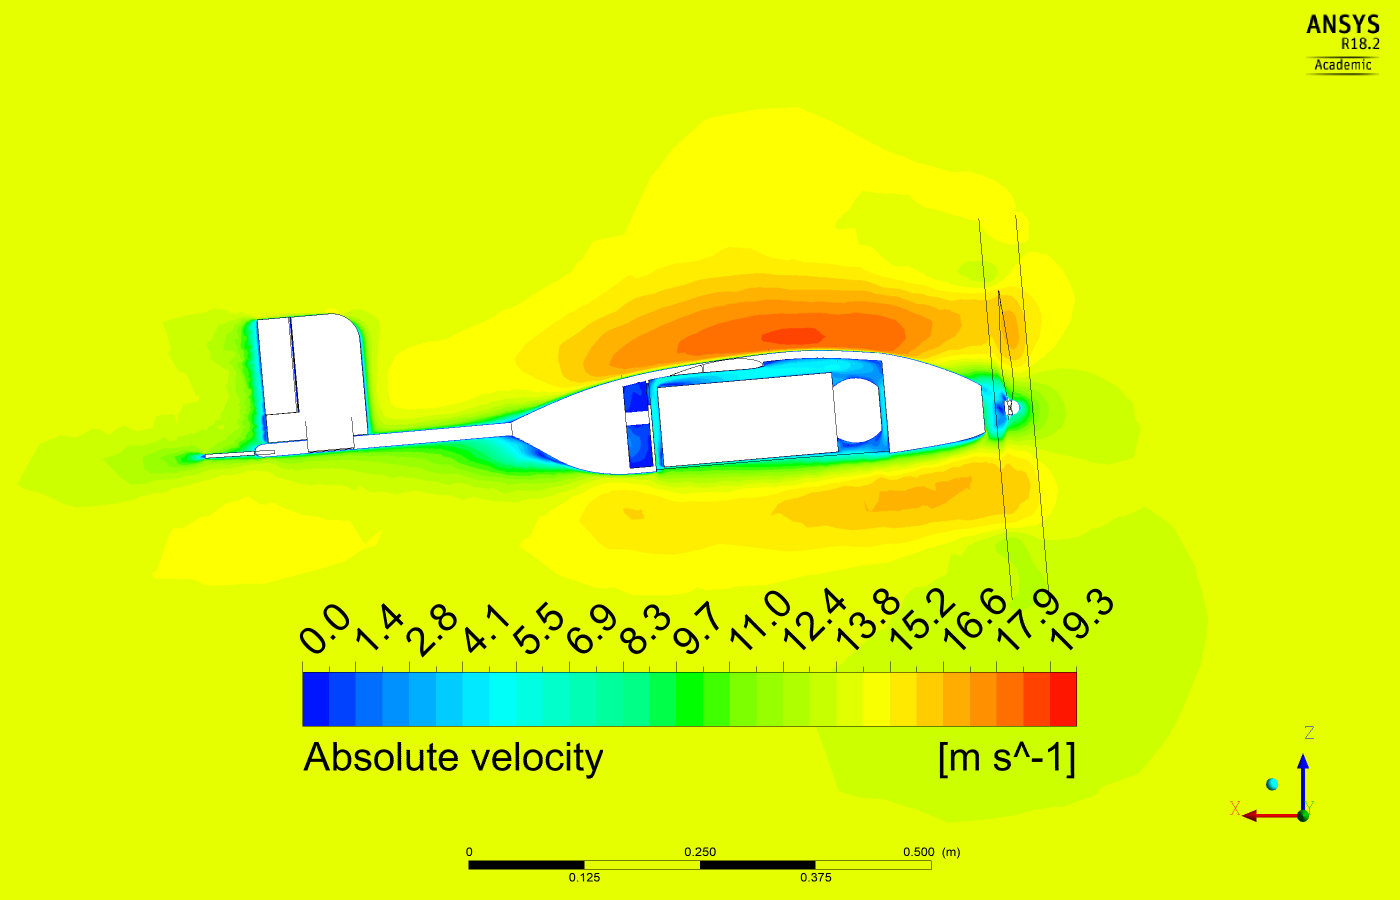
\includegraphics[trim = {6cm 0 8cm 3cm} , clip, width=1\linewidth]{velwbprop.png}
  \captionof{figure}{Velocity contour with added propeller.\label{withprop}}
 \end{minipage}}
\end{figure}

%%%%%%%%%%%%%%%%%%%%%%%%%%%%%%%%  Chapter 5  %%%%%%%%%%%%%%%%%%%%%%%%%%%%%%%%%%%%%%%%%%%
\clearpage
\thispagestyle{plain}
\section{Discussion}
\vspace{.6cm}

A first point that should be brought into discussion is the accuracy of results and uncertainties. Initially, all the simulations were done excluding the propeller which was the biggest unknown in our investigation. The choice for low-order numerical schemes and a coarse mesh (with $y+$ implications) was accepted because we were interested mainly in variations of the parameters and not necessarily in their absolute values. In \cite{ansys} it is mentioned that the overall boundary layer resolution may be more important than a achieving certain $y+$ values. This is why it was tried to have as many cells as possible close to the wall (minimum 10 recommended), even if the resultant $y+$ was not ideal. Moreover, compared to the real aircraft, the differences between the model and CAD and then CFD approximation were huge (for example the wing was covered in plastic film which makes small depressions between the ribs, small but considerable). Despite all these introduced errors, it was shown that the propeller was the missing link. Even if the Moving Reference Frames model assumes that the flow at the exit boundary is sufficiently mixed out and has its own limitations, the effect was enough to prove were the main directional instability came from.

As seen in Figure \ref{np}, after the propeller addition the aircraft is still longitudinally stable, but not directionally stable (Figure \ref{yawmom}). This agrees with the first flight test when a few seconds after launch the aircraft entered a flat spin and became uncontrollable. There was not enough height for the pilot to reduce the power and try to recover the airplane. The physical explanation is that there is a side force component created at the rotor disc as a result of sideslip. This comes from the fact that the incoming air is deflected sideways by the propeller and since the propeller is in front of the CG, it creates a moment which tends to rotate the airplane even more. An indirect effect is that the vertical stabilizer feels mainly the "propwash" and very little the change in sideslip angle, so its ability to produce a restoring moment is diminished. This is why an increase in area of 1.4 (keeping the proportions constant) is less effective with the propeller present than without. This suggests that the tail increase should be done more vertically for two reasons: escape the propeller downwash and not reduce the tail arm. The second flight test was done with a tail 2.6 times bigger and it worked well, so a guess can be made that around a 1.6 tail increase can solve the problem.

A very important remark is that our method to investigate the stability is very primitive and costly. The literature (see the background study and references in \cite{stabil}) is full of methods to calculate stability derivatives, not only static but also dynamic plus their gradients! Mostly it requires specialized codes modified in this sense. Such tools for quick analysis of aircraft stability would be very useful in conceptual design to help decide which configurations are better than others.






%%%%%%%%%%%%%%%%%%%%%%%%%%%%%%%%  Chapter 6  %%%%%%%%%%%%%%%%%%%%%%%%%%%%%%%%%%%%%%%%%%%
\clearpage
\thispagestyle{plain}
\section{Conclusions}

To conclude, we can say that even if the L/D ratio can be improved with 10\% on average by adding a cargo door, it is not worth the mechanical complexity and extra weight. Regarding the stability, a large propeller like the one used can make the difference between "stable" and "unstable". In TMAL06 only the longitudinal stability was calculated. For future projects, definitely calculate all the static stability derivatives to avoid a \emph{crash}! It was also shown that a 1.4 area increase in vertical tail is not enough which suggested that either a taller tail is needed or more area. This study confirms that simple and quick CFD models (like steady state RANS and MRF) are correctly predicting critical behaviour and could be used in aircraft conceptual design.



%%%%%%%%%%%%%%%%%%%%%%%%%%%%%%%%  References %%%%%%%%%%%%%%%%%%%%%%%%%%%%%%%%%%%%%%%%%%
\clearpage
\thispagestyle{plain}

\bibliography{references}
\bibliographystyle{vancouver}

%\putbib[references]
%\end{bibunit}

%%%%%%%%%%%%%%%%%%%%%%%%%%%%%%%%%%%%%%%%%%%%%%%%%%%%%%%%%%%%%%%%%%%





\end{document}

